% vim: fo=aw2tq tw=100
\documentclass[10pt,a4paper]{article}

\usepackage[vmargin=1in,hcentering]{geometry}

\usepackage{hyperref}
\hypersetup{colorlinks=true}

\usepackage{color}
\definecolor{lightgray}{gray}{0.95}

\usepackage{listings}
\lstset{lineskip=-1pt, basicstyle=\small\ttfamily, backgroundcolor=\color{lightgray}, frame=single, 
framerule=0pt}

\usepackage[pdftex]{graphicx}

\usepackage{float}
\restylefloat{figure}

%\setcounter{secnumdepth}{3}

% Hyperlinks suitable for both HTML and PDF
\newcommand{\fhref}[2]{\htmladdnormallinkfoot{#2}{#1}}
% Easier way of using backslash (damn Windows file paths)
\newcommand{\bslash}{\symbol{92}}
% The DO3SE thingy
\newcommand{\DOSE}{{DO$_3$SE}}

\title{\DOSE{} User Guide}
\author{Stockholm Environmental Institute\\
\\
\begin{tabular}{rl}
Contact: & Lisa Emberson (\href{mailto:l.emberson@york.ac.uk}{l.emberson@york.ac.uk})\\
         & Patrick B\"uker (\href{mailto:pb25@york.ac.uk}{pb25@york.ac.uk})
\end{tabular}
}
\date{}


\begin{document}

\maketitle

\newpage

\tableofcontents

\newpage


\section{Main window overview}
\label{sec:overview}

The main window of the \DOSE{} user interface consists of several tabs.  The first of these is a 
short introduction to the \DOSE{} model and the interface; reading this introduction before using 
the model is recommended.  The other tabs allow you to configure various aspects of how the model 
will be run.

\begin{figure}[H]
\centering
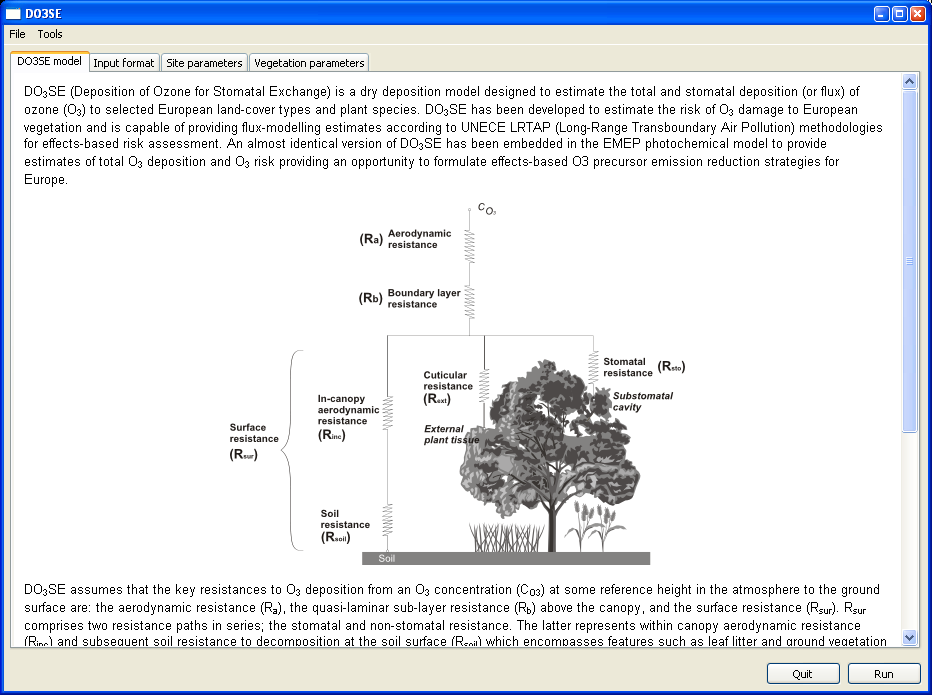
\includegraphics[width=0.5\textwidth]{images/ss/intro-panel}
\end{figure}

\subsection{The ``Input format'' tab}
\label{sec:overview:input}

The ``Input format'' tab allows you to specify the format the input data file is in (see section 
\ref{sec:io-formats}).  This consists of two things: the fields that are present (and their 
ordering), and the number of rows to ignore from the beginning of the file.  This last parameter 
allows headers to be present in the data while not affecting the operation of the model.

\begin{figure}[H]
\centering
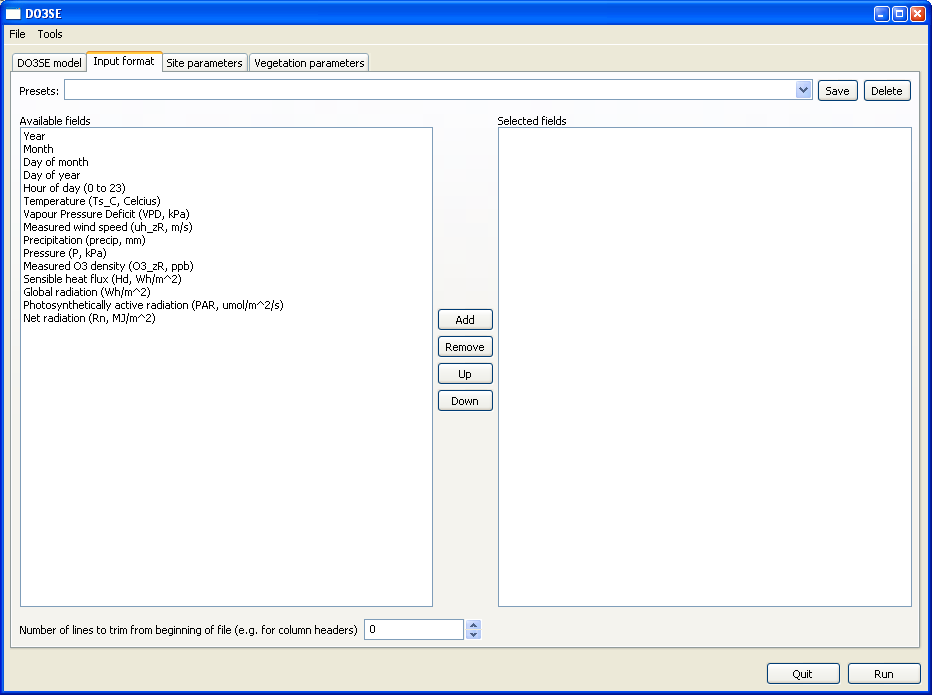
\includegraphics[width=0.5\textwidth]{images/ss/input-format-panel}
\end{figure}


\subsection{The ``Site parameters'' tab}

The ``Site parameters'' tab allows you to specify values for parameters which are properties of the 
location rather than of the vegetation itself such as elevation and heights at which measurements 
are taken.

\begin{figure}[H]
\centering
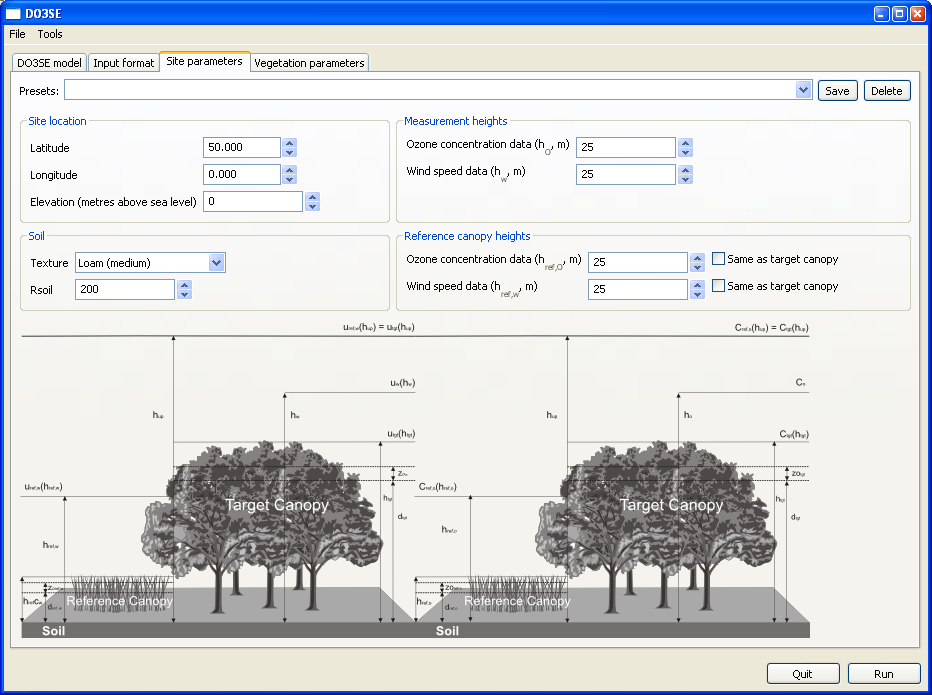
\includegraphics[width=0.5\textwidth]{images/ss/site-params-panel}
\end{figure}


\subsection{The ``Vegetation parameters'' tab}

The ``Vegetation parameters'' tab allows you to specify values for vegetation-specific parameters.  
Since these make up the majority of the parameters, they are further grouped into 3 tabs.

\subsubsection{The ``Characteristics'' tab}

The ``Characteristics'' tab contains constant properties of the vegetation such as albedo and root 
depth.

\begin{figure}[H]
\centering
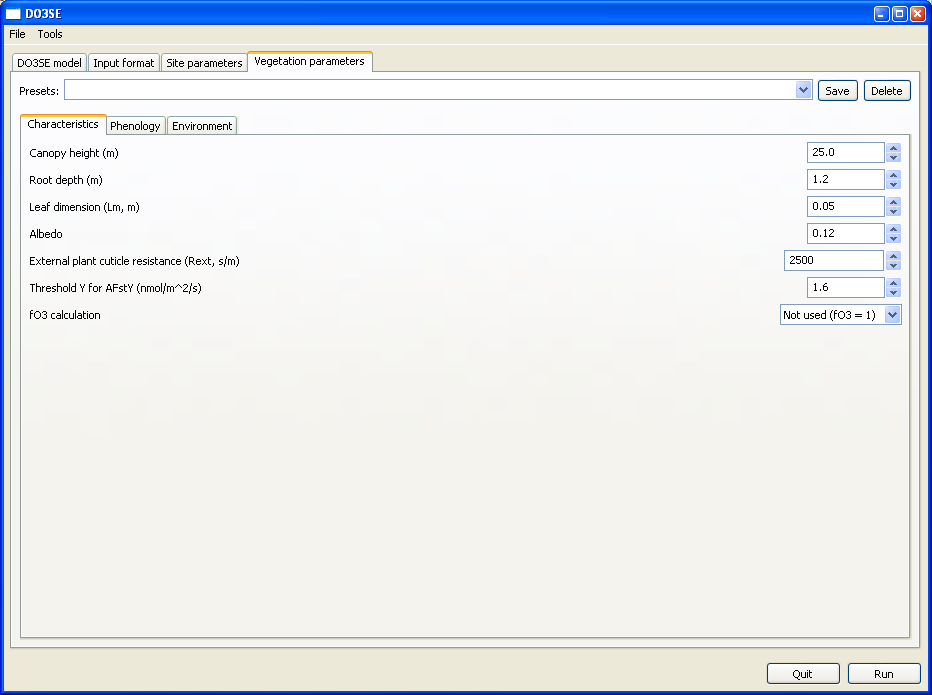
\includegraphics[width=0.5\textwidth]{images/ss/veg-characteristics-panel}
\end{figure}

\subsubsection{The ``Phenology'' tab}

The ``Phenology'' tab defines the functions for Leaf Area Index (LAI), $F_{phen}$ and leaf 
$f_{phen}$.

\begin{figure}[H]
\centering
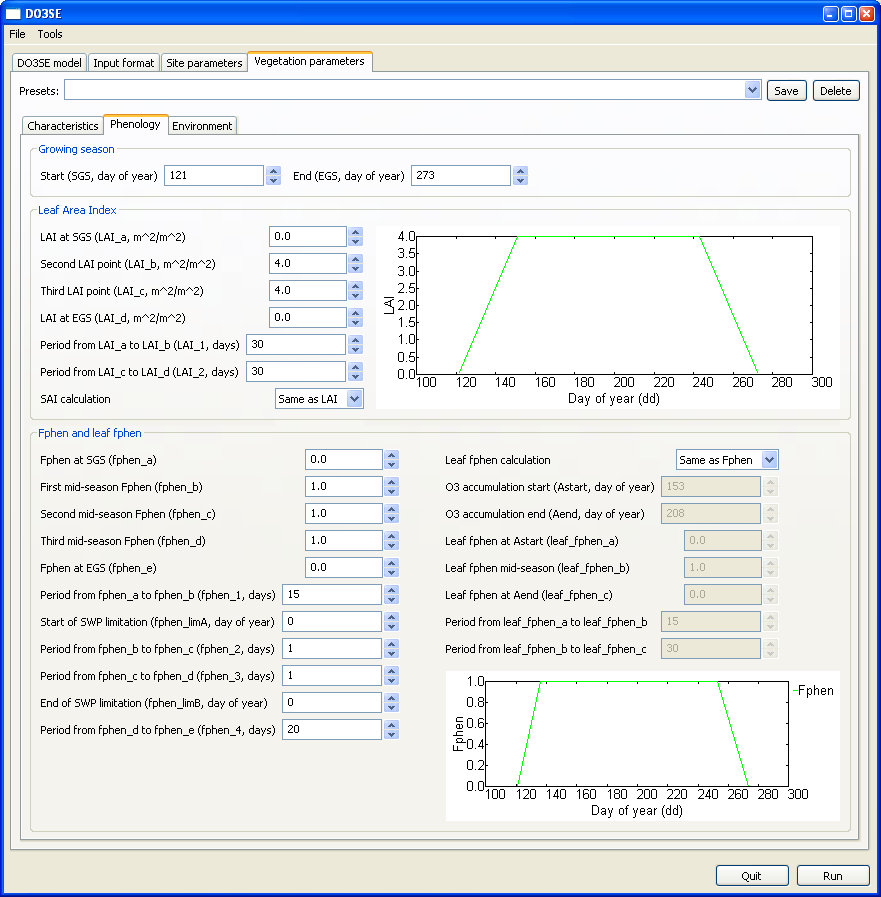
\includegraphics[width=0.5\textwidth]{images/ss/veg-phenology-panel}
\end{figure}

\subsubsection{The ``Environment'' tab}

The ``Environment'' tab contains parameters which define the vegetation's response to particular 
environmental conditions, such as Vapour Pressure Deficit (VPD) and temperature.

\begin{figure}[H]
\centering
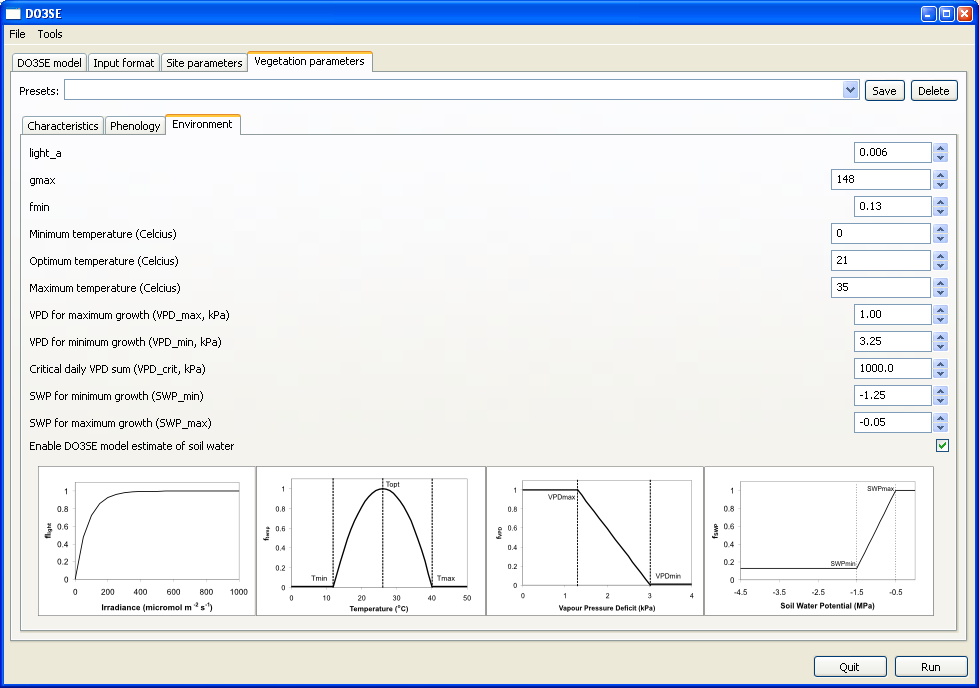
\includegraphics[width=0.5\textwidth]{images/ss/veg-environment-panel}
\end{figure}


\subsection{The ``File'' menu}

\begin{figure}[H]
\centering
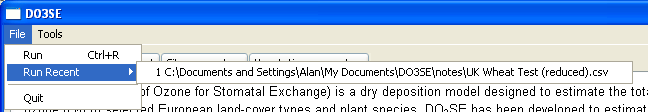
\includegraphics[width=0.7\textwidth]{images/ss/file-menu-cropped}
\end{figure}


\subsection{The ``Tools'' menu}

\begin{figure}[H]
\centering
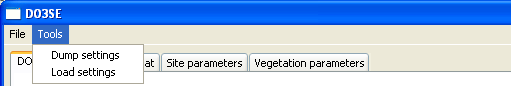
\includegraphics[width=0.7\textwidth]{images/ss/tools-menu-cropped}
\end{figure}



\section{Results window overview}

\subsection{The ``Data'' tab}

\begin{figure}[H]
\centering
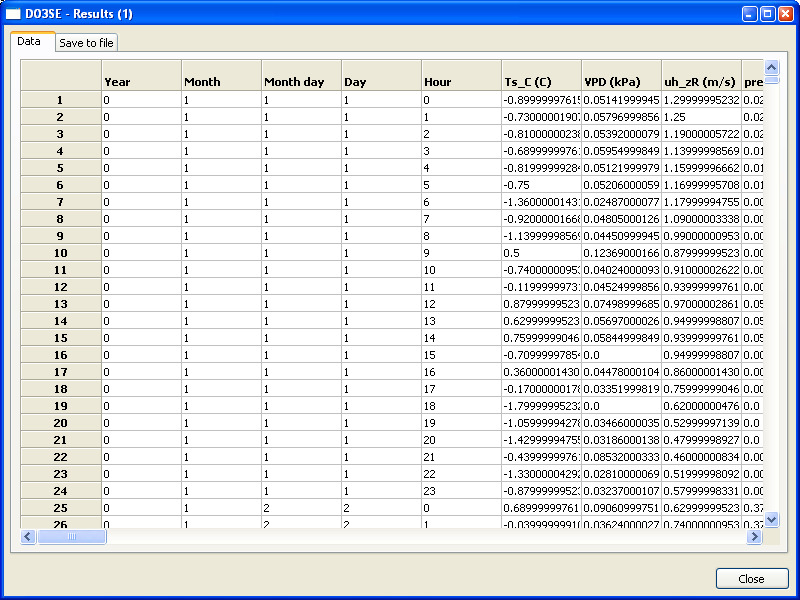
\includegraphics[width=0.5\textwidth]{images/ss/results-grid}
\end{figure}


\subsection{The ``Save to file'' tab}

\begin{figure}[H]
\centering
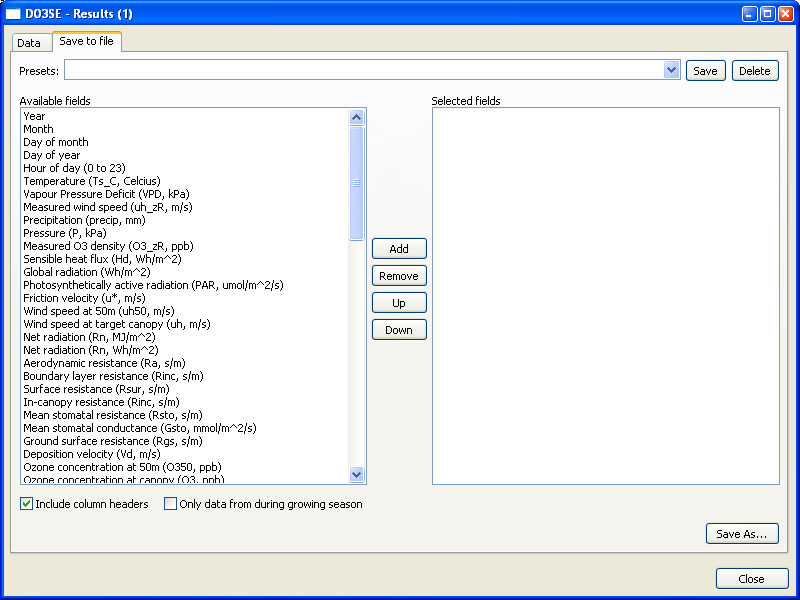
\includegraphics[width=0.5\textwidth]{images/ss/results-save}
\end{figure}



\section{Input and Output Formats}
\label{sec:io-formats}


\end{document}
